\subsection{Definition}

\vspace{-0.5cm}

\begin{figure}[!htb]
\begin{minipage}[t]{0.48\textwidth}
\vspace{-2.5cm}
Based on the example for heat transport in a fluid filled fracture (section \ref{bmt:heat_transport_fracture}), this problem is extended by heat diffusion through a rock matrix orthogonal to the fracture (Fig.~\ref{fig-lauwerier-problem}). 
\end{minipage}
\hspace{0.02\textwidth}
\begin{minipage}[t]{0.48\textwidth}
\centering
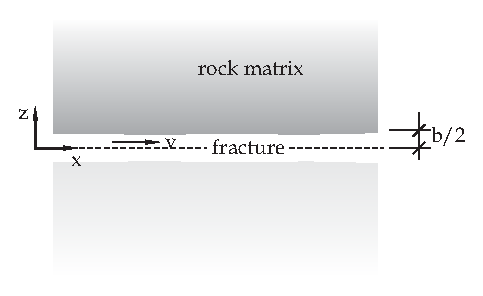
\includegraphics[scale=0.7]{PART_II/T/lauwerier-problem.eps}
\caption{\label{fig-lauwerier-problem} Heat transport in a fracture-matrix system}
\end{minipage}
\end{figure}

The model and material parameters for fracture and rock matrix, respectively, are given in Tab.~\ref{tab-lauwerier-parameters}.

\begin{table}[!htbp]
\caption{\label{tab-lauwerier-parameters}Model parameters for the \textsc{Lauwerier}-problem.}
\begin{center}
\begin{tabular}{llll}
\toprule
Symbol & Parameter & Value & Unit \\
\midrule
\multicolumn{2}{c}{\textit{spatial discretisation}} \\
$L$ & fracture length	& $\unit[50]{}$ & ${m}$  \\
$W$ & matrix width & $\unit[63.25]{}$ & ${m}$  \\
$\Delta x$ & step size X 			& $\unit[2]{}$ & ${m}$  \\
$\Delta z$ & step size Z			& $\unit[0.1265]{}$ & ${m}$  \\
$b/2$ & half of fracture width 	& $\unit[1.0 \cdot 10^{-3}]{}$ & ${m}$  \\
$v_x$ & groundwater velocity 		& $\unit[1.0 \cdot 10^{-4}]{}$ & ${m/s}$ \\
\cmidrule{1-4}
\multicolumn{2}{c}{\textit{temporal discretisation}}\\
$\Delta t$ & time step length 			& $\unit[2.0 \cdot 10^{5}]{}$ & ${s}$  \\ 
& number of timesteps 				& 2500 \\
& total time 						& $\unit[5.0 \cdot 10^{8}]{}$ & ${s}$  \\
\cmidrule{1-4}
\multicolumn{2}{c}{\textit{material properties -- solid}}\\
$\lambda$ & thermal conductivity 	& $\unit[1]{}$ & ${W \cdot m^{-1} \cdot K^{-1}}$  \\
$c$ & heat capacity 				& $\unit[1000]{}$ & ${J \cdot kg^{-1} \cdot K^{-1}}$  \\
$\rho$ & density 					& $\unit[2500]{}$ & ${kg \cdot m^{-3}}$  \\
\cmidrule{1-4}
\multicolumn{2}{c}{\textit{material properties -- fluid}}\\
$c$ & heat capacity 				& $\unit[4000]{}$ & ${J \cdot kg^{-1} \cdot K^{-1}}$  \\
$\rho$ & density 					& $\unit[1000]{}$ & ${kg \cdot m^{-3}}$  \\
\bottomrule
\end{tabular}
\end{center}
\end{table}

\subsection{Solution}

For this problem an analytical solution was derived by \textsc{Lauwerier} (1955) (see \cite{Kol:97}) with following assumptions:
\begin{compactitem}
\item in the fracture, heat is transported only by advection,
\item in the rock matrix, heat transport takes place by diffusion (only along the z-axis).
\end{compactitem}
The \textsc{Lauwerier} solution is given by
%
\begin{equation}
T_D=\begin{cases}
0, & t_D < x_D \\
\operatorname{erfc}\left\{ \frac{\beta}{\sqrt{\alpha\left(t_D-x_d\right)}} \left[ x_D+\frac{1}{2\beta}\left( z_D-\frac{1}{2} \right) \right]\right\}, & t_D > x_D
\end{cases},   z_D \geq\frac{1}{2}
\label{lauwerier}
\end{equation}
%
with the following dimensionless parameters:
%
\begin{equation}
t_D=\frac{v_x}{b}t,\ \ \ x_D=\frac{x}{b},\ \ \ z_D=\frac{z}{b},\ \ \ \alpha =\frac{\lambda ^{s}}{c^{s}\rho ^{s}}\frac{1}{bv_x},\ \ \ \beta = \frac{\lambda^{s}}{c^{l}\rho^{l}}\frac{1}{bv_x}
\end{equation}
%
where $b$ is the fracture width, $\lambda$ is the thermal conductivity, $c$ is the heat capacity, $\rho$ is the density and the suffixes $s$ and $f$ denote the solid (rock) and liquid (water) phases, respectively.

The numerical \textsc{Lauwerier} model is formed as a coupling of advective 1D heat transport in x-direction and diffusive 1D heat transport in z-direction. This means, that nodes in the rock matrix are not influenced by their left or right neighbors. The matrix elements are connected to the fracture elements orthogonally. Fig.~\ref{fig-lauwerier-grid} shows a schematical description of the model setup. Because of the symmetry, the numerical model calculates just the domain above the x-axis. 

\begin{figure}[htbp!]
\centering
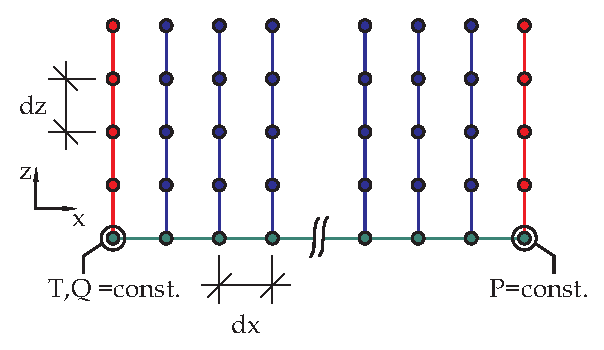
\includegraphics[width=0.65\textwidth]{PART_II/T/lauwerier-grid.eps}
\caption{\label{fig-lauwerier-grid}Alignment of the grid for the numerical model.}
\end{figure}

Fig.~\ref{fig-lauwerier-scheme} shows the positions of observation points which were chosen to evaluate the numerical model by the comparison with analytical solutions. 
%
\begin{figure}[!htbp]
\centering
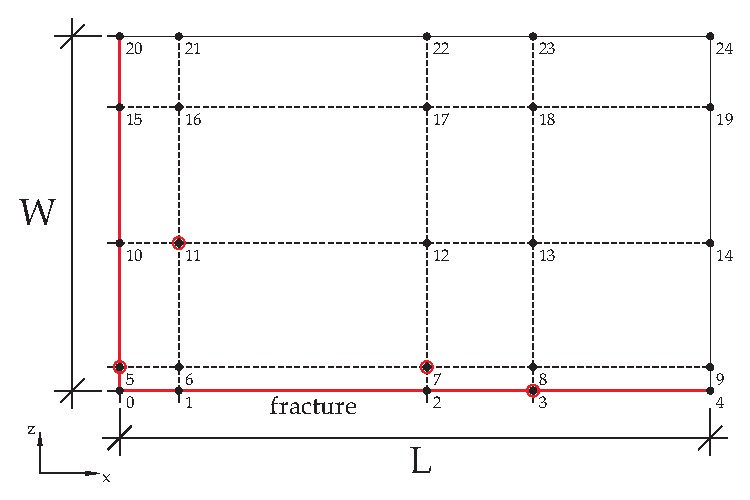
\includegraphics[width=0.65\textwidth]{PART_II/T/lauwerier-scheme.eps}
\caption{\label{fig-lauwerier-scheme}Positions of observation points for temperature breakthrough curves.}
\end{figure}

\begin{figure}[H]
\centering
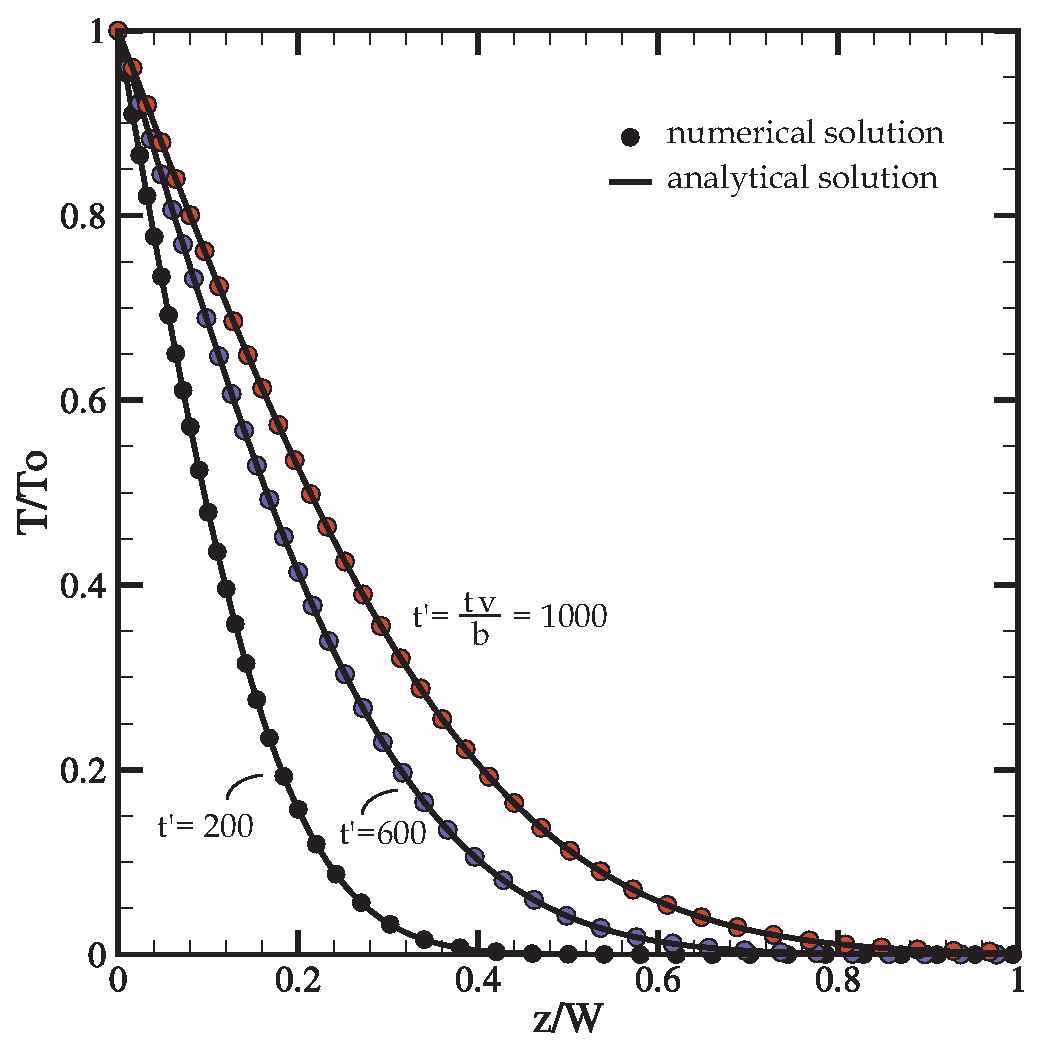
\includegraphics[width=0.6\textwidth]{PART_II/T/lauwerier-rock.eps}
\caption{Temperature distribution orthogonal to the fracture at $x=0$ at three different times.}
\label{fig-lauwerier-rock}
\end{figure}

\subsection{Results}

The quality of the numerical results can be shown by temperature distribution curves for several times in the rock matrix. Fig.~\ref{fig-lauwerier-rock} shows the temperature profiles for $x=\unit[0]{m}$ at three moments $t'$. The numerical solution has a very good agreement to the analytical results. Temperature profiles along the fracture at $z=\unit[0]{m}$ are plotted in Fig.~\ref{fig-lauwerier-fracture}. 

\begin{figure}[!htbp]
\centering
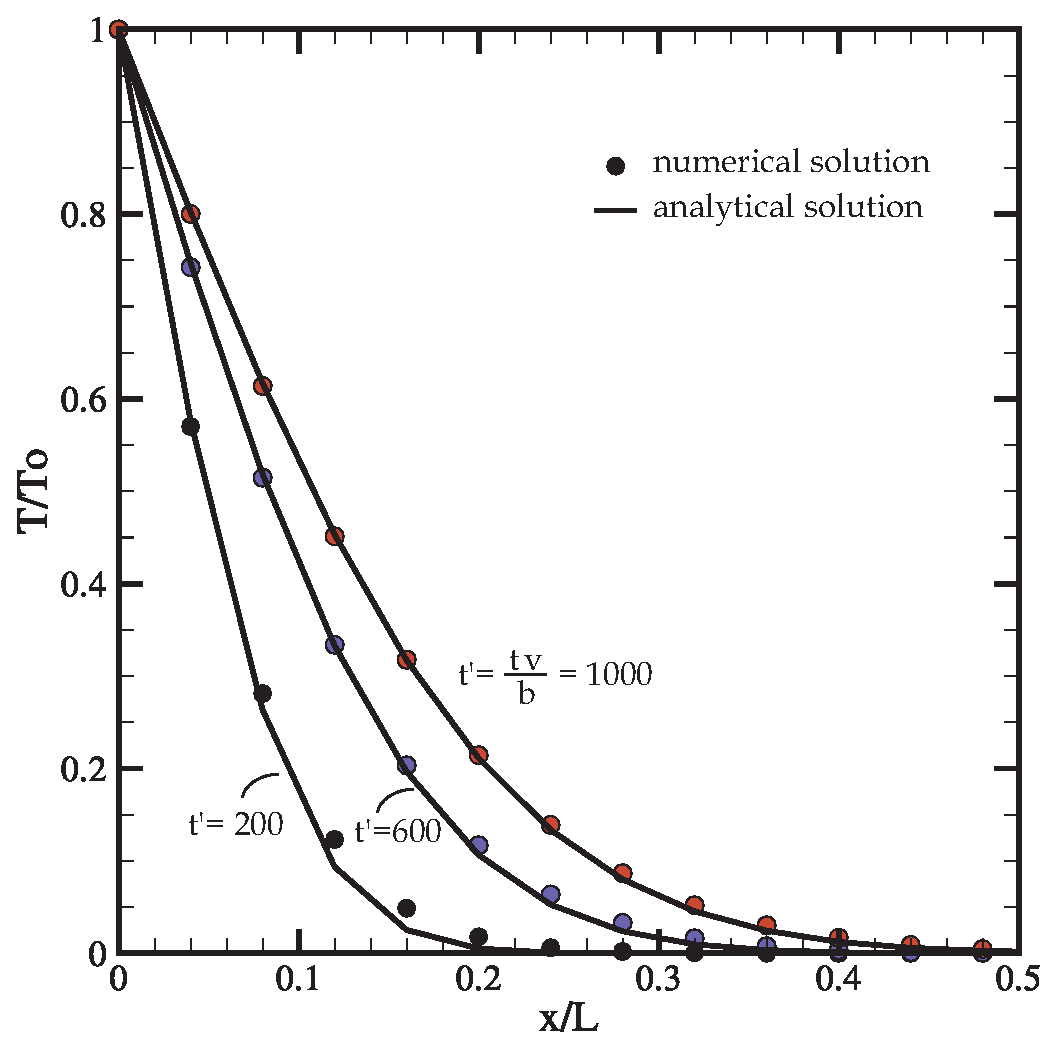
\includegraphics[width=0.6\textwidth]{PART_II/T/lauwerier-fracture.eps}
\caption{Temperature distribution along the fracture at three different times.}
\label{fig-lauwerier-fracture}
\end{figure}

\begin{figure}[!htbp]
\centering
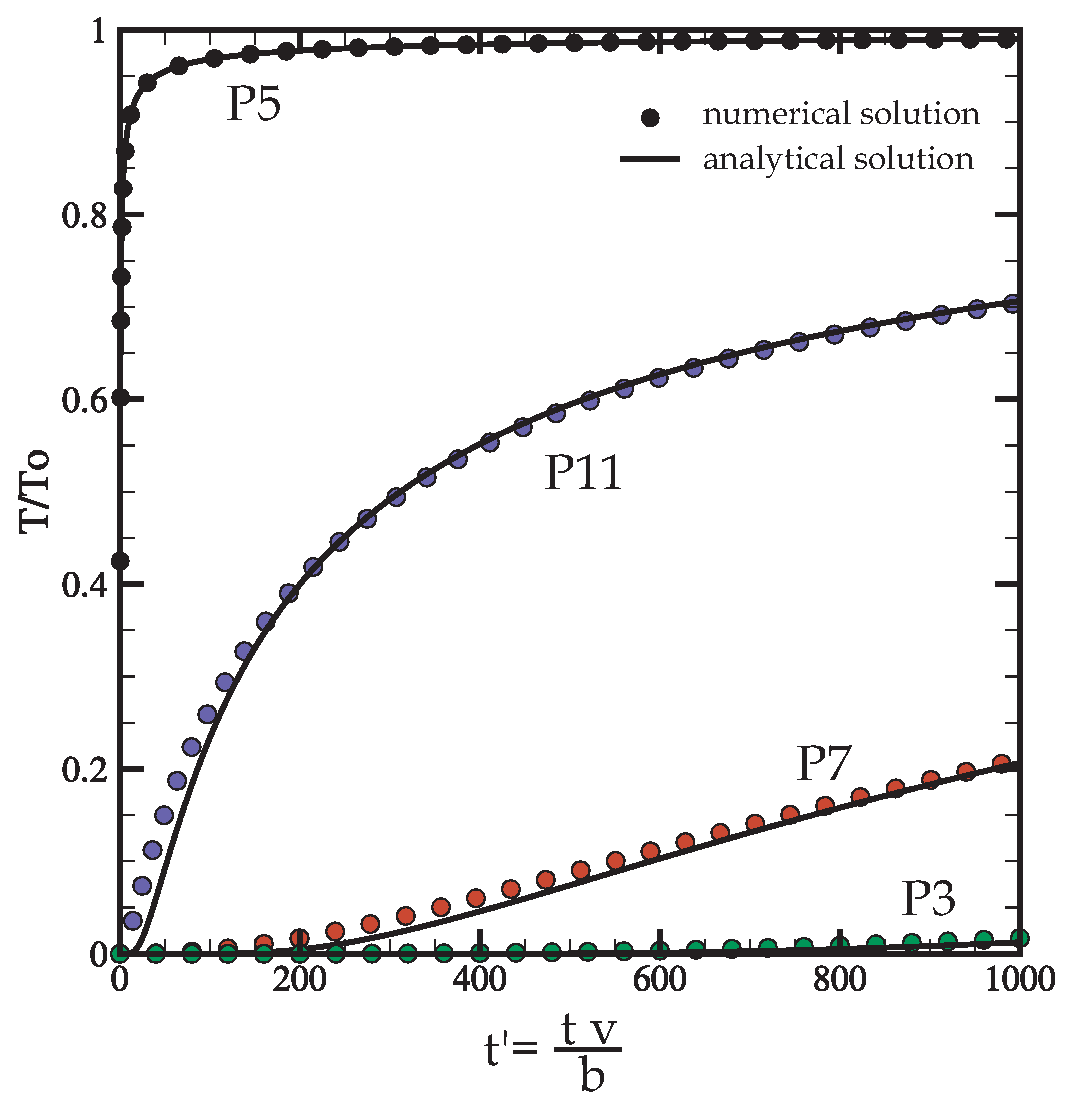
\includegraphics[width=0.6\textwidth]{PART_II/T/lauwerier-points.eps}
\caption{Temperature breakthrough curves at certain points in the rock matrix.}
\label{fig-lauwerier-points}
\end{figure}

For long simulation times ($t'=1000; t'=600$) both solutions fits very well together. For short simulation times, the numerical solution differ slightly from the analytical results. This discrepancy for short simulation times can be examined in Fig.~\ref{fig-lauwerier-points}, where temperature breakthrough curves for certain points (see Fig.~\ref{fig-lauwerier-scheme}) is plotted.

%\clearpage
